\documentclass[babel={layout=lists},9pt]{beamer-rl}
\usepackage{subcaption}
\usepackage{setspace}
\usepackage{nicefrac}
\usepackage{tikz}
\usepackage{amsmath,mathtools}
\usepackage[absolute,overlay]{textpos}
\usepackage{graphicx}
\usepackage{booktabs}
\usepackage{multirow}
\usepackage[font=scriptsize,labelfont=bf]{caption}
\usepackage{algorithm2e}
\usepackage{tcolorbox,xcolor}
\newtcolorbox{mybox}{colback=MSUgreen!50,boxrule=0pt,arc=0pt,left=0pt,right=0pt,top=2pt,bottom=2pt,boxsep=0pt,width=2.2cm}

\usetikzlibrary{quotes}
\usetikzlibrary{arrows}

\usefonttheme[onlymath]{serif}
\babelprovide[import,main,mapdigits]{persian}
\babelfont{sf}{XB Zar}


% برخی تم قابل استفاده. ویرایشات انجام شده در ادامه، برای قالب برکلی است
\mode<presentation>{\usetheme[width=2.2cm,hideothersubsections]{Berkeley}}
%\mode<presentation>{\usetheme[width=2.2cm,hideothersubsections]{PaloAlto}}
%\mode<presentation>{\usetheme[width=2.2cm,hideothersubsections]{Goettingen}}

\usecolortheme{spruce} %رنگ  بندی قالب 

% تعریف رنگ سبز زیبا برای تم
\definecolor{MSUgreen}{RGB}{46, 139, 87}  % سبز زمردی (Seagreen)
%\definecolor{MSUgreen}{RGB}{60, 179, 113} % سبز متوسط (MediumSeaGreen)
%\definecolor{MSUgreen}{RGB}{34, 139, 34}  % سبز جنگلی (ForestGreen)
%\definecolor{MSUgreen}{RGB}{0, 128, 0}    % سبز (Green)


%%%% اضافه کردن هایلایت به سکشن فعال در سایدبار و اعمال چند رنگ بندی دیگر
\setbeamercolor{palette sidebar secondary}{fg=black,bg=MSUgreen!50} 
\setbeamercolor{subsection in sidebar}{fg=MSUgreen!50!black}
\setbeamercolor{section in sidebar shaded}{fg=white}
\setbeamercolor{title in sidebar}{fg=white}
\setbeamercolor{author in sidebar}{fg=black}
\setbeamercolor{navigation symbols}{fg=gray}
\setbeamercolor{frame number}{bg=MSUgreen!50,fg=black}

% تنظیم رنگ های مختلف بلاک ها با سبز جدید
\setbeamercolor{block title}{fg=white,bg=black!5!MSUgreen}
\setbeamercolor{block body}{fg=black,bg=white!90!MSUgreen}
\setbeamercolor{block title example}{fg=white,bg=black!5!MSUgreen}
\setbeamercolor{block body example}{fg=black,bg=white!90!MSUgreen}
\setbeamercolor{block title theorem}{fg=white,bg=black!5!MSUgreen}
\setbeamercolor{block body theorem}{fg=black,bg=white!90!MSUgreen}
\setbeamercolor{block title definition}{fg=white,bg=black!5!MSUgreen}
\setbeamercolor{block body definition}{fg=black,bg=white!90!MSUgreen}
\setbeamercolor{block title proof}{fg=white,bg=black!5!MSUgreen}
\setbeamercolor{block body proof}{fg=black,bg=white!90!MSUgreen}

% تنظیم رنگ آیتم ها با سبز جدید
\setbeamercolor{itemize item}{fg=MSUgreen!60!black}
\setbeamercolor{itemize subitem}{fg=MSUgreen!40!black}
\setbeamercolor{itemize subsubitem}{fg=MSUgreen!20!black}

\setbeamercolor{enumerate item}{fg=MSUgreen!60!black}
\setbeamercolor{enumerate subitem}{fg=MSUgreen!40!black}
\setbeamercolor{enumerate subsubitem}{fg=MSUgreen!20!black}
\setbeamercolor{item projected}{bg=MSUgreen!20!black,fg=white}

% تنظیم شکل آیتم ها
\setbeamertemplate{itemize item}[square]
\setbeamertemplate{itemize subitem}[circle]
\setbeamertemplate{itemize subsubitem}[triangle]

% تنظیم سربرگ و پانل ها با سبز جدید
\setbeamercolor{section in head/foot}{bg=MSUgreen!90!black,fg=white}
\setbeamercolor{subsection in head/foot}{bg=MSUgreen!80!black,fg=white}
\setbeamercolor{palette primary}{bg=MSUgreen,fg=white}
\setbeamercolor{palette secondary}{bg=MSUgreen!80!black,fg=white}
\setbeamercolor{palette tertiary}{bg=MSUgreen!60!black,fg=white}
\setbeamercolor{palette quaternary}{bg=MSUgreen!40!black,fg=white}
\setbeamercolor{frametitle}{bg=MSUgreen!90!black,fg=white}


%%%%% کوچک کردن سایز فونت فرمول ها
\makeatletter
\DeclareMathSizes{9}{8}{7}{7} % first parameter should be equal to beamer-rl font size
\makeatother




%%%%%% افزایش مارجین سکشن ها در سایدبار

\makeatletter


\setbeamertemplate{subsection in sidebar}{%
	\beamer@sidebarformat{5pt}{subsection in sidebar}{• \insertsubsectionhead}% افزودن بالت به ساب سکشن
}

\def\insertverticalnavigation#1{%
	\setstretch{1.3}
	\vbox{%
		\def\sectionentry##1##2##3##4##5{%
			\ifnum##5=\c@part%
			\def\insertsectionhead{##2}%
			\def\insertsectionheadnumber{##1}%
			\def\insertpartheadnumber{##5}%
			\hbox to #1{{%
					\usebeamerfont{section in sidebar}\usebeamercolor[fg]{section in sidebar}%
					\hyperlink{Navigation##3}{%
						\ifnum\c@section=##1%
						\ifnum\c@subsection=0\relax%
						{\usebeamertemplate{section in sidebar}}%
						\else%
						\ifx\beamer@nav@css\beamer@hidetext%
						{\usebeamertemplate{section in sidebar}}%
						\else%
						{\usebeamertemplate{section in sidebar shaded}}%
						\fi%
						\fi%
						\else
						{\usebeamertemplate{section in sidebar shaded}}%
						\fi}}}%
			\vskip2pt %%%% افزودن فاصله
			\beamer@currentsubsection=0\relax\fi}%
		\def\slideentry##1##2##3##4##5##6{}%
		\def\beamer@subsectionentry##1##2##3##4##5{%
			\ifnum##1=\c@part%
			\def\insertpartheadnumber{##1}%
			\def\insertsectionheadnumber{##2}%
			\def\insertsubsectionheadnumber{##3}%
			\def\insertsubsectionhead{##5}%
			\beamer@tocifnothide{\ifnum\c@section=##2\ifnum\c@subsection=##3\beamer@nav@css\else\beamer@nav@oss\fi\else\beamer@nav@ooss\fi}%
			{\hbox{{%
						\usebeamerfont{subsection in sidebar}\usebeamercolor[fg]{subsection in sidebar}%
						\hspace{1pt}
						\hyperlink{Navigation##4}{%
							\ifnum\c@section=##2%
							\ifnum\c@subsection=##3%
							\ifnum\c@subsubsection=0\relax%
							{\usebeamertemplate{subsection in sidebar}}%
							\else%
							{\usebeamertemplate{subsection in sidebar shaded}}%
							\fi%
							\else%
							{\usebeamertemplate{subsection in sidebar shaded}}%
							\fi%
							\else%
							{\usebeamertemplate{subsection in sidebar shaded}}%
							\fi}}}%
			}%
			\fi}%
		\def\beamer@subsubsectionentry##1##2##3##4##5##6{%
			\ifnum##1=\c@part%
			\def\insertpartheadnumber{##1}%
			\def\insertsectionheadnumber{##2}%
			\def\insertsubsectionheadnumber{##3}%
			\def\insertsubsubsectionheadnumber{##4}%
			\def\insertsubsubsectionhead{##6}%
			\beamer@tocifnothide{\ifnum\c@section=##2\ifnum\c@subsection=##3\ifnum\c@subsubsection=##4\beamer@nav@css\else\beamer@nav@oss\fi\else\beamer@nav@ooss\fi\else\beamer@nav@ooss\fi}%
			{\hbox{{%
						\usebeamerfont{subsubsection in sidebar}\usebeamercolor[fg]{subsubsection in sidebar}%
						\hyperlink{Navigation##5}{%
							\ifnum\c@section=##2%
							\ifnum\c@subsection=##3%
							\ifnum\c@subsubsection=##4%
							{\usebeamertemplate{subsubsection in sidebar}}%
							\else
							{\usebeamertemplate{subsubsection in sidebar shaded}}%
							\fi%
							\else%
							{\usebeamertemplate{subsubsection in sidebar shaded}}%
							\fi%
							\else%
							{\usebeamertemplate{subsubsection in sidebar shaded}}%
							\fi}}}%
			}%
			\fi}%
		%\beamer@currentsubsection=0\relax%
		\dohead%
	}%
}

\makeatother

%%%%% افزودن شماره صفحه به اسلاید
% برای تغییر محل شماره صفحه 0,9.25 را تغییر دهید

\setbeamertemplate{footline}{%
	
	\begin{textblock*}{2cm}(0cm,9.25cm)
		\begin{mybox}
			\centering
			{\footnotesize
				\textcolor{MSUgreen!60!black}{\insertframenumber/\inserttotalframenumber}
			}
		\end{mybox}
	\end{textblock*}
	
	\vskip0pt%
}

% تنظیم عنوان بخش ها
\AtBeginSection[]{
	\begin{frame}
		\vfill
		\centering
		\begin{beamercolorbox}[sep=8pt,center,shadow=true,rounded=true]{palette secondary}
			\usebeamerfont{title}\insertsectionhead\par%
		\end{beamercolorbox}
		\vfill
	\end{frame}
}

\AtBeginSubsection[]{
	\begin{frame}
		\vfill
		\centering
		\begin{beamercolorbox}[sep=8pt,center,shadow=true,rounded=true]{title}
			\usebeamerfont{title}\insertsubsectionhead\par%
		\end{beamercolorbox}
		\vfill
	\end{frame}
}


\uselanguage{persian}
\languagepath{persian}
\deftranslation[to=persian]{Theorem}{قضیه}
\deftranslation[to=persian]{theorem}{قضیه}
\deftranslation[to=persian]{Corollary}{نتیجه}
\deftranslation[to=persian]{corollary}{نتیجه}
\deftranslation[to=persian]{Definition}{تعریف}
\deftranslation[to=persian]{definition}{تعریف}
\deftranslation[to=persian]{Definitions}{تعاریف}
\deftranslation[to=persian]{definitions}{تعاریف}
\deftranslation[to=persian]{Fact}{حقیقت}
\deftranslation[to=persian]{fact}{حقیقت}
\deftranslation[to=persian]{Example}{مثال}
\deftranslation[to=persian]{example}{مثال}
\deftranslation[to=persian]{Examples}{مثال‌ها}
\deftranslation[to=persian]{examples}{مثال‌ها}
\deftranslation[to=persian]{Lemma}{لم}
\deftranslation[to=persian]{lemma}{لم}
\deftranslation[to=persian]{Table}{جدول}
\deftranslation[to=persian]{table}{جدول}


\newcommand*{\Scale}[2][4]{\scalebox{#1}{$#2$}}%
\newcommand*{\Resize}[2]{\resizebox{#1}{!}{$#2$}}%
\newcommand\crule[3][black]{\textcolor{#1}{\rule{#2}{#3}}}

\title{عنوان اسلاید}
\author{نویسنده}
\institute{نام دانشگاه}
\date{تاریخ}
\logo{
\includegraphics[width=1.1cm]{assets/logo}}

\begin{document}
	
	
	\begin{frame}[noframenumbering,plain]
		
\includegraphics[width=7 cm]{assets/Besmellah.png}
		\begin{textblock*}{13cm}(0cm,9cm)
			\crule[MSUgreen]{13cm}{1cm}
		\end{textblock*}
	\end{frame}
	
	
	
	\begin{frame}
		\maketitle
	\end{frame}
	\begin{frame}
		\frametitle{فهرست مطالب}
		\hfill
		\parbox[t]{.95\textwidth}{
			%\begin{minipage}[c][0.75\textheight]{\textwidth} % افزایش فاصله عمودی بین عنوان فصل ها
			{
				\setcounter{tocdepth}{1} 
				\tableofcontents
			}
			%\end{minipage}
		}
	\end{frame}
	
	
	
	\section{فصل اول}
	
	
	\begin{frame}
		\frametitle{عنوان اسلاید}
		\framesubtitle{زیر عنوان اسلاید}
		\begin{itemize}
			\setlength\itemsep{1em} % تنظیم فاصله عمودی بین آیتم ها
			\item آیتم اول
			\item آیتم دوم
			\item آیتم سوم
			\vspace{0.5em} % افزایش فاصله 
			\begin{itemize}
				\setlength\itemsep{1em}
				\item زیر آیتم اول
				\item زیر آیتم دوم
				\vspace{0.5em} % افزایش فاصله 
				\begin{itemize}
					\setlength\itemsep{1em}
					\item زیر زیر آیتم اول
					\item زیر زیر آیتم دوم
				\end{itemize}
			\end{itemize}
		\end{itemize}
	\end{frame}
	
	
	\subsection{زیر فصل اول}
	
	
	\begin{frame}
		\frametitle{اسلاید دوم}
		در اینجا یک متن برای تست و در زیر یک فرمول ریاضی
		\begin{equation*}
		a x + b = 0
		\end{equation*}
		قرار دارد.
	\end{frame}
	
	
	\begin{frame}
		\frametitle{اسلاید سوم}
		
		\begin{definition}[عنوان تعریف]
			متن تعریف
		\end{definition}
		
		\vspace{15pt} % فاصله عمودی
		
		\begin{theorem}[عنوان قضیه]
			متن قضیه
		\end{theorem}
		
		\begin{example}[شماره مثال]
			متن مثال
		\end{example}
		
	\end{frame}
	
	\begin{frame}
		\frametitle{اسلاید چهارم}
		اسلاید دو ستونه
		\begin{columns}[T] 
			\begin{column}{.48\textwidth}
				\vspace{30pt}
				\begin{equation*}
				\Scale[0.85]{ % تغییر اندازه کل فرمول ها
					\begin{aligned}
					1+1=2
					\end{aligned}
				}
				\end{equation*}
			\end{column}
			\hfill
			\begin{column}{.48\textwidth}
				\begin{figure}
					\centering
					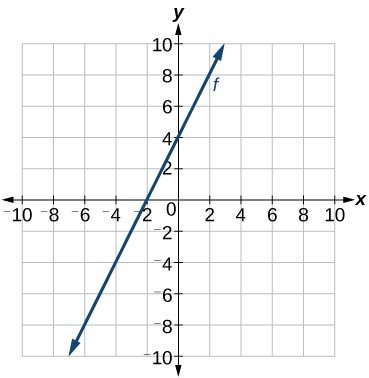
\includegraphics[width=1\linewidth]{assets/plot.jpg}
					\caption{نمودار یک}
				\end{figure}
			\end{column}
		\end{columns}
	\end{frame}
	
	
	
	\begin{frame}
		\frametitle{اسلاید پنجم}
		
		{\selectlanguage{nil}
			An English text.
		}
	\end{frame}
	
	
	\section{فصل دوم}
	
	\begin{frame}
		\frametitle{عنوان اسلاید}
		\begin{exampleblock}{}
			{
				یک جعبه برای نقل قول متن
			}
			\vskip5mm
			\hspace*\fill{\small--- اسم}
		\end{exampleblock}
	\end{frame}
	
	
	
	\begin{frame}
		\frametitle{عنوان اسلاید}
		قرار دادن شکل در محل دلخواه
		\begin{textblock*}{3cm}(4cm,6cm) % {block width} (coords)
			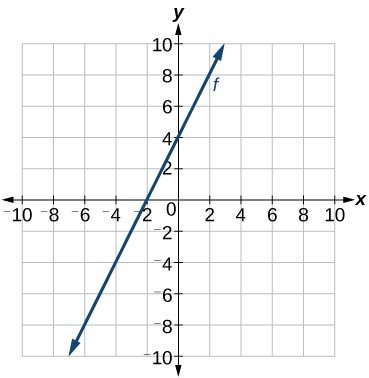
\includegraphics[width=3cm]{assets/plot.jpg}
		\end{textblock*}
		
	\end{frame}
	
	
	
	\begin{frame}
		\frametitle{رسم شکل}
		
		
		\begin{tikzpicture}
		
		\hskip-0.7cm
		
		\tikzset{vertex/.style = {shape=circle,draw,minimum size=1.5em}}
		\tikzset{edge/.style = {->,> = latex'}}
		
		
		\node[vertex] (A) at  (5,1.5) [text width=1cm,align=center] {A};
		\node[vertex] (B) at  (2,-3) [text width=1cm,align=center] {B};
		\node[vertex] (C) at  (8,-3) [text width=1cm,align=center] {C};
		
		\draw[->] (A) -- (C);
		\draw[->] (C) -- (A);
		\draw (A) -- (C)  node [midway, above, sloped] (TextNode) {A};
		\draw (A) -- (C)  node [midway, below, sloped] (TextNode) {C};
		
		
		
		\draw[->] (A) -- (B);
		\draw[->] (B) -- (A);
		\draw (A) -- (B)  node [midway, above, sloped] (TextNode) {A};
		\draw (A) -- (B)  node [midway, below, sloped] (TextNode) {B};
		
		\draw[->] (B) -- (C);
		\draw[->] (C) -- (B);
		\draw (B) -- (C)  node [midway, above, sloped] (TextNode) {BC};
		
		\end{tikzpicture}
		
		
	\end{frame}
	
	
	\begin{frame}
		\begin{beamercolorbox}[sep=8pt,center,shadow=true,rounded=true]{palette secondary}
			پایان
		\end{beamercolorbox}
	\end{frame}
	
\end{document}